
\paragraph{Имплементация паразитного поля}\label{chpt3:imperfections:implementation}
Имплементируя неидеальности полей, мы следовали рекомендациям
изложенным в~\cite[стр.~235]{Eremey:Thesis}. Малое возмущение
магнитного поля, в первом приближении, действует как маленький пропорциональный поворот
спин-вектора (спин-кик). Поэтому мы имплементировали наклон E+B элемента как
домножение соответствующей матрицы поворота на его спиновую трансфер-матрицу.
Такая имплементация наклона элемента гарантирует сохранение 
замкнутой орбиты; физически, сохранение замкнутой орбиты обусловлено 
появлением компенсирующего электрического поля спин-ротатора при его наклоне.

В соответствии с уравнением~\eqref{eq:TBMT_MDM}, изменение МДМ частоты
прецессии, ассоциированное с введённым паразитным полем $(B_x, 0, B_z)$ есть
\begin{align*}
	\Delta\W_{MDM} &= \frac qm G \cdot (B_x, 0, B_z),
	\intertext{поэтому угол спин-кика равен}
	\Theta_{kick} &= t_0\Delta\W_{MDM},
\end{align*}
где $t_0 = L/v_0$ пролётное время референсной частицы через элемент.

\subsection{Зависимость от распределения неидеальностей} \label{chpt3:imperfections:magnitude}
Данная серия симуляций была проведена с целью подтвердить два тезиса
касательно систематической ошибки измерения частоты прецессии спина вокруг
радиальной оси, вызванной неточностью установки E+B элементов:
\begin{enumerate*}[(1)]
	\item индуцированный МДМ-эффект зависит только от среднего значения
	угла наклона элементов, но не от  конкретной последовательности
	углов; и
	\item эта зависимость носит линейный характер.
\end{enumerate*}

Симуляция была проведена следующим образом: мы распределили наклоны
$\Theta_{tilt}$ E+B элементам FS структуры случайным образом. После
построения трансфер-матриц (спиновой и орбитальной) до  3-го порядка разложения Тэйлора, 
были вычислены разложения Тэйлора функций спин-тюна и оси прецессии спина (SPA). Члены нулевого
порядка последних представляют собой спин-тюн и SPA референсной частицы.

Угловая скорость поворота спин-вектора референсной частицы вычисляется по формуле:~\cite[стр.~4]{COSY:SpinTuneMapping}
\[
\vec\W = 2\pi/\tau_0\cdot \nu_s \cdot \bar n,
\]
где $\tau_0 = f^{-1}_{rev} = 10^{-6}$ секунд есть пролётное время частицы через ускоритель.

Симуляция была проведена 11 раз. Каждый раз углы наклона
спин-ротаторов выбирались из нормального распределения
$N(\mu_0\cdot(i-5), \sigma_0)$, где ${\mu_0 = 10\cdot \sigma_0 =10^{-4}}$~рад, 
${i\in\lbrace0,\dots, 10\rbrace}$. Результаты представлены
на Рисунке~\ref{fig:Linearity_test_shifting_gauss}.

\begin{figure}[H]
	\centering
	\subbottom[Компоненты оси прецессии $\nbar$]{%
		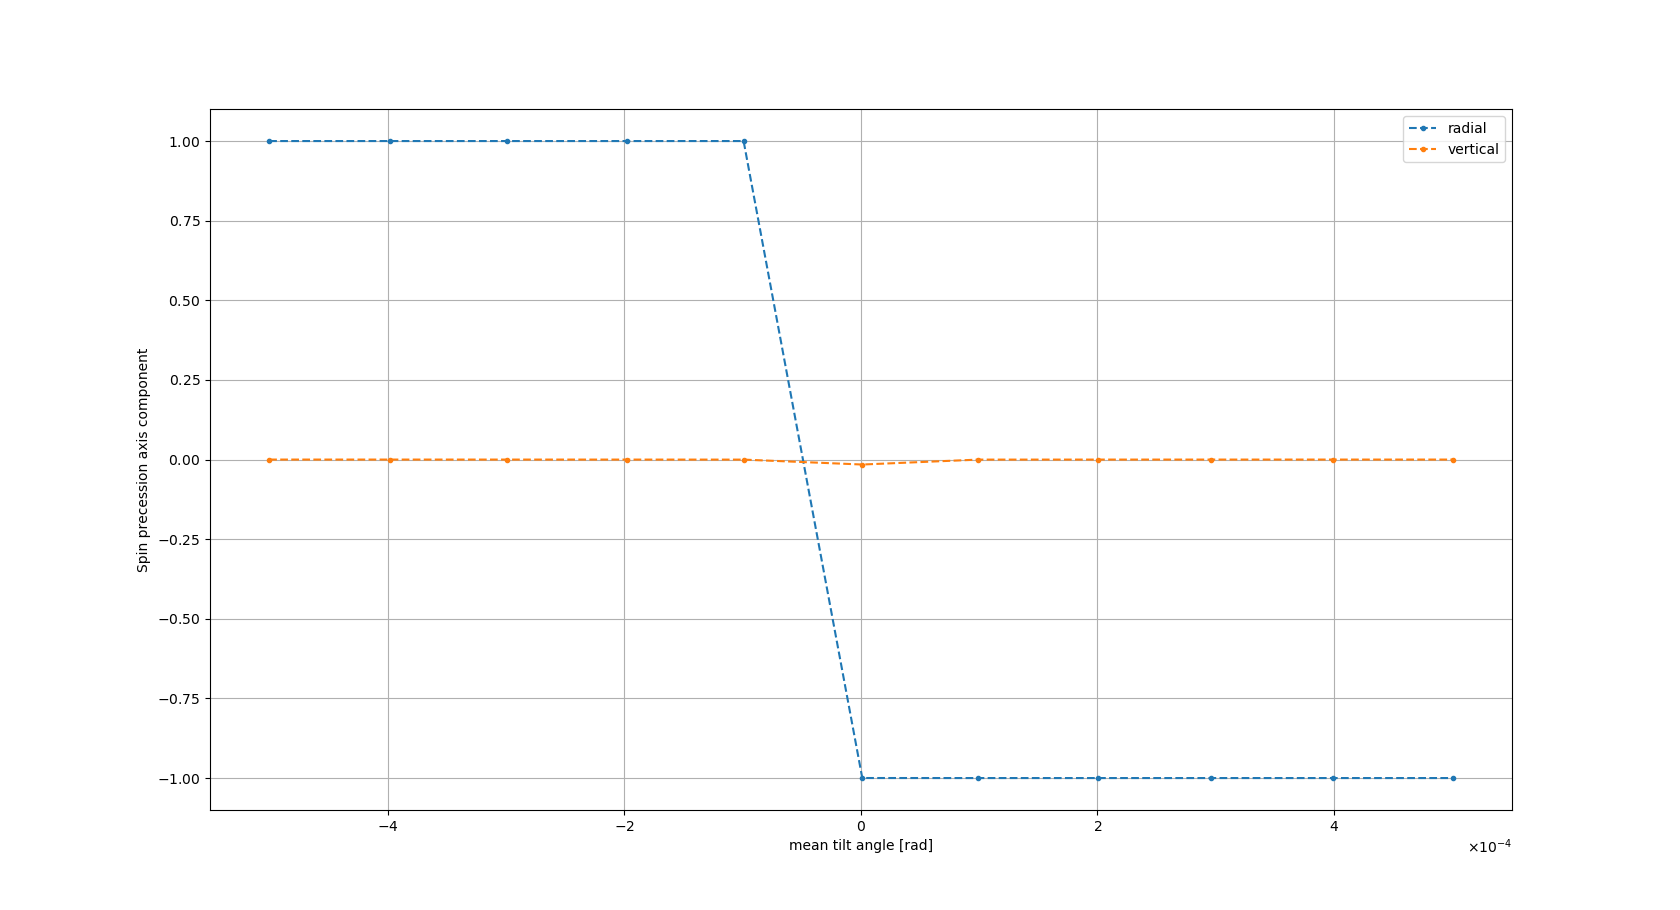
\includegraphics[height=.35\paperheight]{images/fake_signal_sim/linearity_test_shifting_gauss_nbar}}
\end{figure}
\begin{figure}[H]\centering
	\contsubbottom[Компоненты частоты прецессии $\vec\W$]{%
		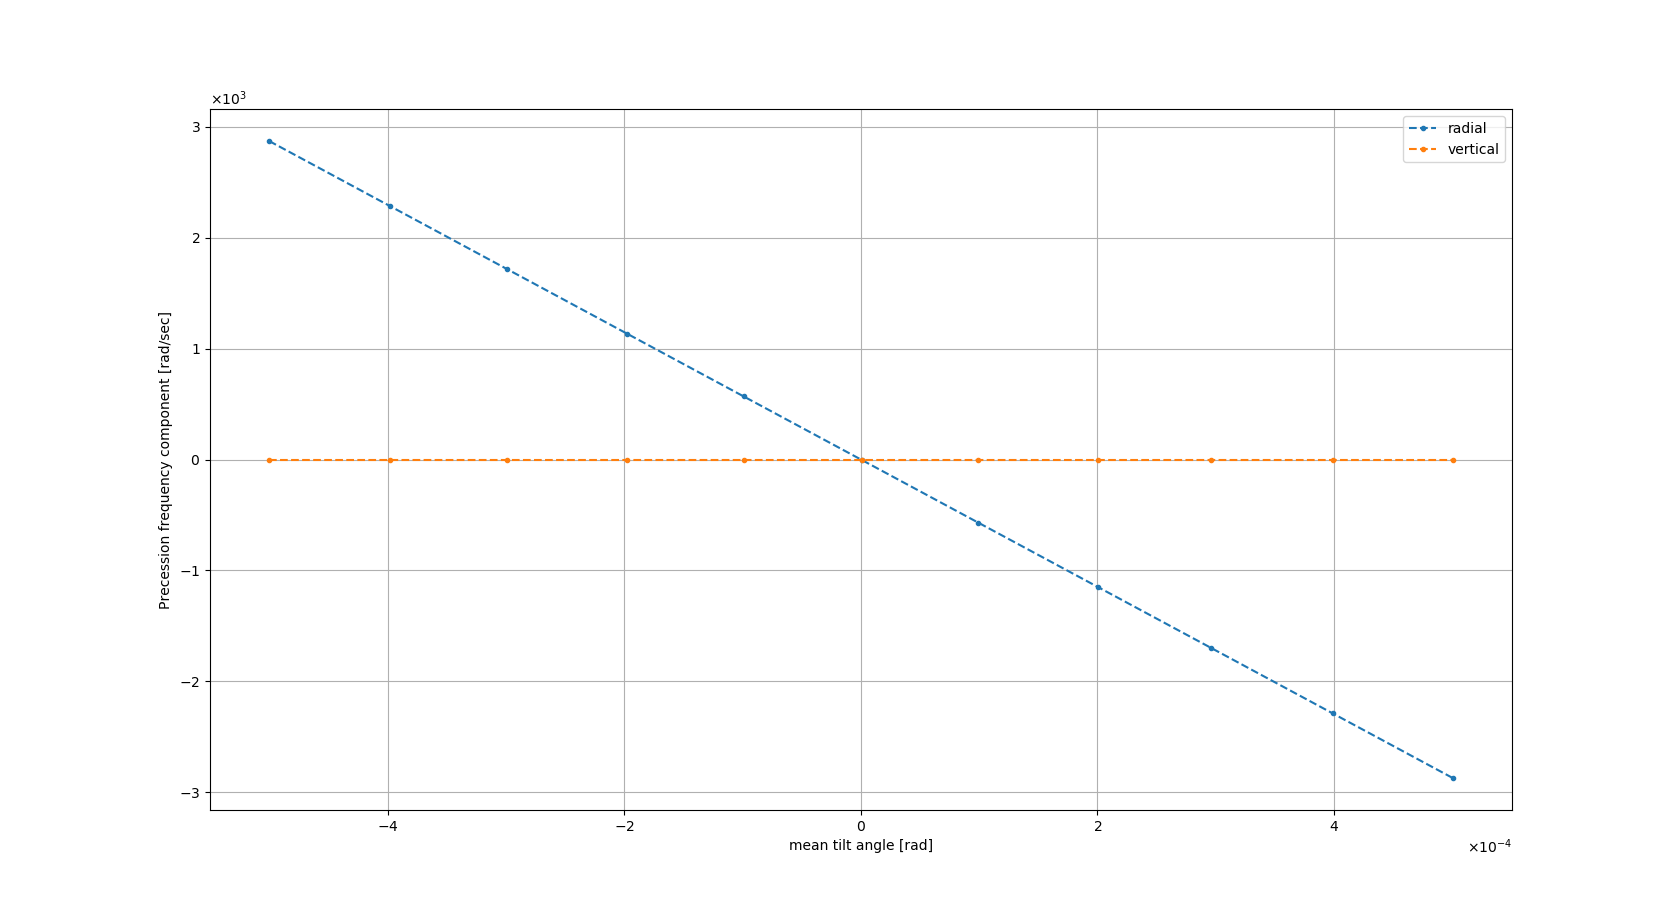
\includegraphics[height=.35\paperheight]{images/fake_signal_sim/linearity_test_shifting_gauss_freq}}
	\legend{Цветом различаются радиальная (синий) и вертикальная (оранжевый) компоненты векторов $\bar n$, $\vec\W$.}
	\caption{Зависимость направления и частоты прецессии спина референсной частицы в неидеальной FS-структуре со случайно-распределёнными ошибками установки спин-ротаторов от их среднего угла наклона.\label{fig:Linearity_test_shifting_gauss}}
\end{figure}

Из рисунка видно, что при такой установке элементов, при которой среднее значение угла наклона равно 
$10^{-4}$~рад, поляризация пучка будет вращаться в вертикальной плоскости с угловой срокостью 
около 500~рад/сек. Это согласуется с оценками выше (раздел~\ref{chpt3:imperfections},
 ур-е~\eqref{eq:tilted-MDM-precession-freq}), поскольку в них предполагается 
 стандартное отклонение ошибки наклона $10^{-4}$~рад, а также наклон ${n=100}$ элементов. 
 В этом случае, стандартное отклонение среднего угла наклона элементов равно $10^{-5}$~рад, и значит, 
 с вероятностью 67\%, МДМ спин-прецессия вокруг радиальной оси будет происходить со скоростью 
 до 50~рад/сек, а с вероятностью 95\% --- до 100~рад/сек.

На Рисунке~\ref{fig:Linearity_test_compensated} изображены результаты теста, в котором 
E+B элементы попарно повёрнуты на противоположные углы (три случайные пары), а один элемент 
повёрнут на угол ${\mu_i = (i-5)\cdot 10^{-6}}$ рад, ${i\in\lbrace0,\dots,10\rbrace}$. Обе симуляции были 
выполнены на энергии 270.0092~МэВ.\footnote{На этой энергии, в идеальной структуре, 
	$\nu_s$ и $\nbar$ не определены в системе координат связанной с пучком, используемой в
	COSY INFINITY. Это соответствует ситуации, когда спин не прецессирует ни в какой плоскости 
	(горизонтальной или вертикальной), что есть условие трёхмерно-замороженного спина, 
	для идеальной структуры.} Можно наблюдать, что скомпенсированные элементы не дают вклад во вращение
спин-вектора референсной частицы.

\begin{figure}[H]
	\centering
	\subbottom[Компоненты оси прецессии $\nbar$]{%
		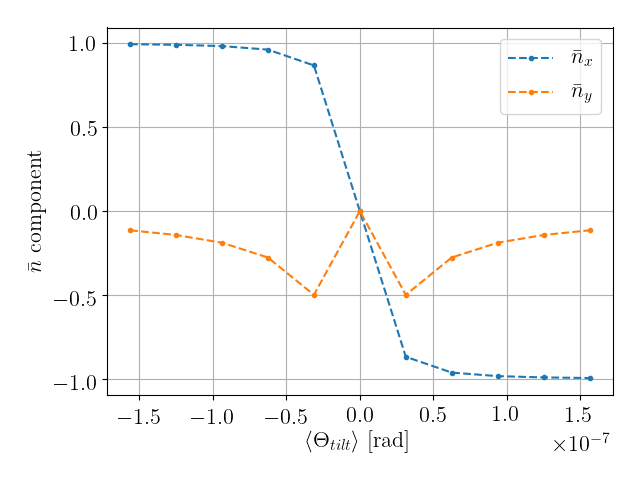
\includegraphics[height=.35\paperheight]{images/fake_signal_sim/linearity_test_compensated+microrad_nbar}}
\end{figure}
\begin{figure}[H]\centering
	\contsubbottom[Компоненты частоты прецессии $\vec\W$]{%
		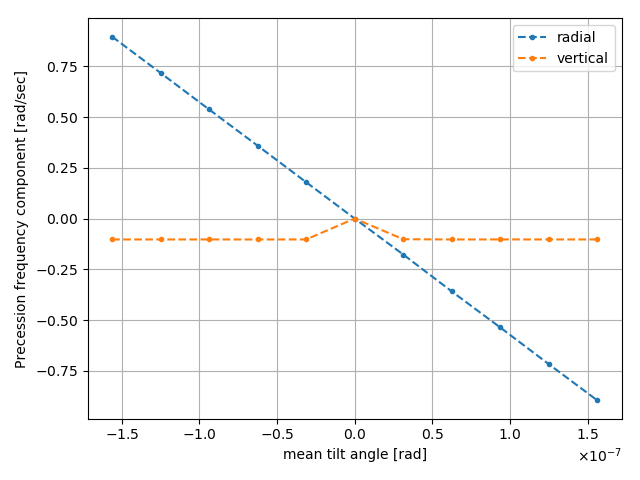
\includegraphics[height=.35\paperheight]{images/fake_signal_sim/linearity_test_compensated+microrad_freq}}
	\caption{Зависимость направления и частоты прецессии спина референсной частицы в неидеальной FS-структуре в случае попарно-компенсированных ошибок установки спин-ротаторов от их среднего угла наклона.\label{fig:Linearity_test_compensated}}
\end{figure}



\subsection{Равенство частот прецессии спинов частиц при движении в прямом и обратном направлениях}\label{chpt3:imperfections:CW_vs_CCW}
На Рисунке~\ref{fig:Lin_test_rel_diff} изображена относительная разница между значениями
радиальной компоненты оси стабильного спина $\nbar_x$ (частоты спин-прецессии $\W_x$) частицы, 
при движении пучка по часовой (CW) или против часовой (CCW) стрелки, соответственно для случаев 
случайно-распределённой ошибки наклона элементов, и при попарной компенсации наклонов.

Для радиальной компоненты оси стабильного спина, относительная разница вычислялась как 
\[
\delta\nbar_x = \frac{\nbar_x^{CW}(\avg{\Theta_{tilt}}) - \nbar_x^{CCW}(\avg{\Theta_{tilt}})}{\nbar_x^{CW}(\avg{\Theta_{tilt}})};
\]
для частоты, соответственно:
\[
\delta\W_x = \frac{\W_x^{CW}(\avg{\Theta_{tilt}}) - \W_x^{CCW}(\avg{\Theta_{tilt}})}{\W_x^{CW}(\avg{\Theta_{tilt}})}.
\]

Из рисунков следует, что при движении пучка в любом из направлений, ось стабильного спина 
наклонена одинаково; при этом существует \emph{различие} между спин-тюнами CW и CCW пучков, но 
на уровне не более десятых долей процента, которое тем сильнее, чем меньше модуль частоты спин-прецессии. 
Эта \emph{разница}  свидетельствует об асимметричности ускорительной структуры 
относительно обращения направления движения, с точки зрения спиновой динамики, 
и может объясняться различием референсных орбит прямого и обратного пучков. 

\begin{figure}[H]
	\centering
	\subbottom[Случайно-распределённые наклоны E+B элементов]{%
		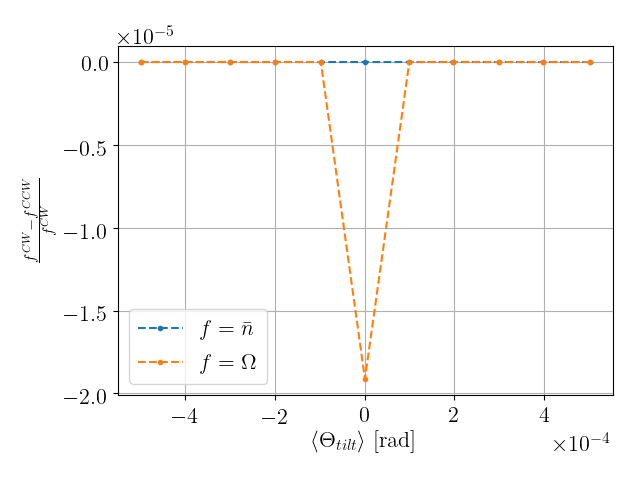
\includegraphics[height=.35\paperheight]{images/fake_signal_sim/linearity_test_shifting_gauss_rel_diff}	
	}
\end{figure}
\begin{figure}[H]\centering
	\contsubbottom[Попарно-компенсированные наклоны]{%
		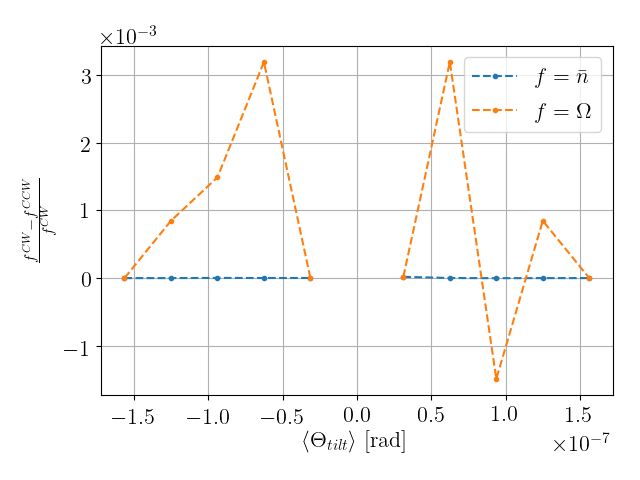
\includegraphics[height=.35\paperheight]{images/fake_signal_sim/linearity_test_compensated+microrad_rel_diff}
	}
	\legend{Цветом обозначена разница между радиальными компонентами (синий) оси стабильного спина, (оранжевый) частоты спин-прецессии CW и CCW пучков}
	\caption{Относительная разница между радиальными компонентами оси стабильного спина и угловой скоростью поворота спина, посчитанная относительно значения для CW-циркулирующего пучка\label{fig:Lin_test_rel_diff}}
\end{figure}
